\documentclass{article}
\usepackage{amsmath}
\usepackage{graphicx}
\usepackage{subfig}


\begin{document}
\title{PP4 Report}
\author{Logan Bontrager}
\maketitle

\section*{Task 1)}

The top five words for each topic are shown below where each line corresponds to a topic and the words are presented in decreasing order.
\\ \\
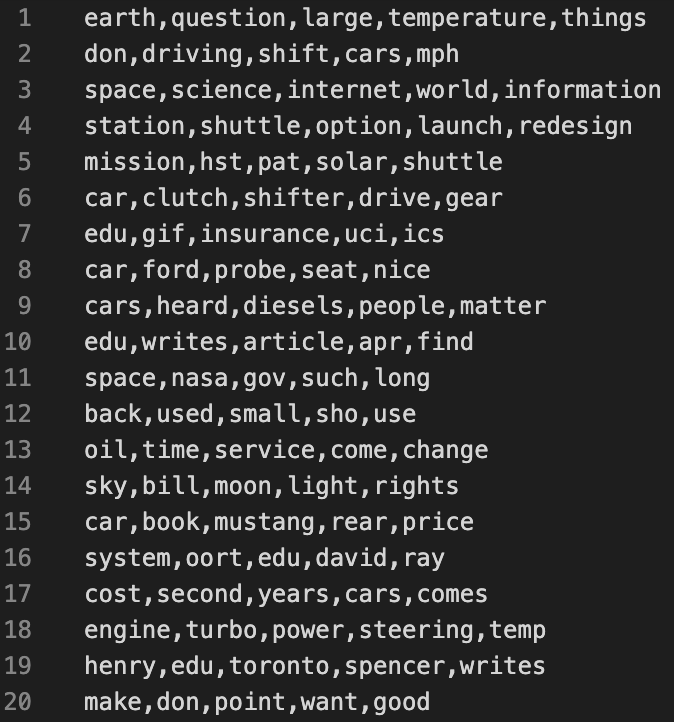
\includegraphics[width=0.8\textwidth]{../output/topics.png}
\\ \\
Here, we can see that most topics have well defined themes. It appears that the two underlying topics present in the data are cars and space. One thing that sticks out to me about the model is that some words carry more weight in terms of human theme definition than others. For example, topic one contains the word things which doesn't have much weight in terms of personal interprepability although I suppose it could be useful in other ways.

\section*{Task 2)}

The graphs below show the test error vs. training size for the bayesian logistic regression model trained on both the topic representation data and the bag of words. we can see that both datasets performance similarly. The main disticintion is that the topic representation data appears to preform better on smaller training sizes than the bag of words. This could be advantageous under data scarcity. The error bars from each graph look rather consistent with each other given the y scale.
\\ \\
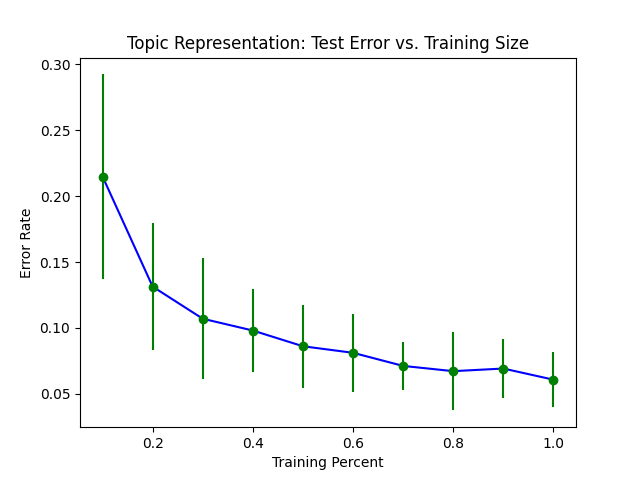
\includegraphics[width=0.6\textwidth]{../output/t2-topic.png}
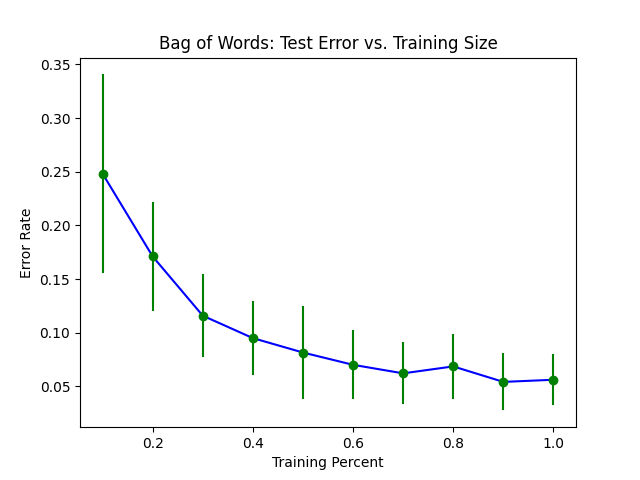
\includegraphics[width=0.6\textwidth]{../output/t2-bag.png}
\\ \\



\end{document}